\documentclass[12pt]{article}
\usepackage{amsmath}
\usepackage{graphicx}

\title{Word Count MapReduce Implementation}
\author{Group Project}
\date{3/12/2024}

\begin{document}

\maketitle

\begin{abstract}
This report describes the implementation of a Word Count problem using a Python-based MapReduce-like approach. The program utilizes multi-threading and synchronization to efficiently count the frequency of words across multiple input text files. The tasks were divided among five group members for collaborative work.
\end{abstract}

\section{Introduction}
The Word Count problem is a classic example of distributed computing, where the goal is to count the frequency of each word in a large collection of text. Our implementation employs Python's threading module and shared data structures to simulate a MapReduce framework. The tasks were divided among group members as follows:
\begin{itemize}
    \item \textbf{Vu Hai Thien Long:} Implemented the core logic for cleaning and processing words.
    \item \textbf{Luu Linh Ly:} Designed the multi-threading structure for processing files concurrently.
    \item \textbf{Nguyen Ngoc Nhi:} Implemented thread-safe mechanisms using locks.
    \item \textbf{Le Viet Hoang Lam:} Created the functionality for saving results to the output folder.
    \item \textbf{Nguyen Duc Duy:} Managed integration and testing of the overall program.
\end{itemize}

\section{Choice of MapReduce Implementation}
The decision to implement this problem in Python with threading was motivated by the following considerations:
\begin{itemize}
    \item \textbf{Ease of Implementation:} Python's threading module provides a simple interface for concurrent execution.
    \item \textbf{Efficiency:} Multi-threading allows parallel processing of files, reducing runtime.
    \item \textbf{Thread Safety:} Shared data structures are protected using locks, ensuring correctness in concurrent operations.
    \item \textbf{Scalability:} The approach can handle multiple files simultaneously, making it suitable for moderate-sized datasets.
\end{itemize}

\section{Mapper and Reducer}
In our implementation, the Mapper and Reducer roles are defined as follows:

\subsection{Mapper}
The Mapper function, \texttt{count\_words\_in\_file}, is responsible for:
\begin{itemize}
    \item Reading a file line by line.
    \item Splitting lines into words.
    \item Cleaning words by converting them to lowercase and removing punctuation.
    \item Counting word occurrences locally using a dictionary.
\end{itemize}

\subsection{Reducer}
The Reducer functionality merges the local dictionaries from all threads into a global word count map. This process is synchronized using a lock to ensure thread safety. The final output is a comprehensive word frequency map across all input files.

\section{Flowchart of the Process}
\begin{figure}[h!]
\centering
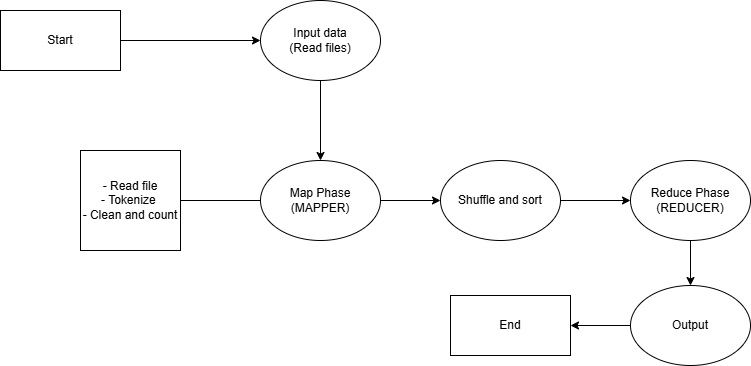
\includegraphics[width=0.8\textwidth]{mapred_flowchart.png}
\caption{Flowchart of the Mapper and Reducer process.}
\label{fig:flowchart}
\end{figure}

\section{Conclusion}
This implementation demonstrates the effectiveness of a Python-based MapReduce-like framework for solving the Word Count problem. The use of threading and locks ensures efficient and thread-safe processing of multiple files. This collaborative project allowed us to learn and apply parallel programming concepts in Python.

\end{document}
